\documentclass{article}

% import packages
\usepackage{amsmath,amsfonts,amsthm,amssymb,amsopn,bm}
\usepackage{mathtools}
\usepackage[margin=.9in]{geometry}
\usepackage{graphicx}
\usepackage[dvipsnames]{xcolor}
\usepackage{minted}
\usepackage{subcaption}
\usepackage{float}

% note command
\newcommand{\note}[1]{\textsf{\textcolor{Red}{#1}}}

% some math commands
\newcommand{\norm}[1]{\left\|#1\right\|}
\newcommand{\twonorm}[1]{\|#1\|_2^2}
\newcommand{\vect}[1]{\boldsymbol{#1}} % vector 
\DeclareMathOperator{\E}{\mathbb{E}}
\DeclareMathOperator{\D}{\mathcal{D}}
\DeclareMathOperator{\cov}{Cov}
\DeclareMathOperator{\var}{Var}

% remove indents
\setlength\parindent{0px}
% enumerate with lowercase letters
\renewcommand{\theenumi}{\textbf{\alph{enumi}}}
% indented environment for solutions
\usepackage{changepage}
\newenvironment{solution}{\begin{adjustwidth}{8mm}{}}{\end{adjustwidth}}


% Homework title and date
\renewcommand{\title}{Homework 0 A}
\renewcommand{\date}{October 5, 2020}

\begin{document}

\begin{center}
        \LARGE \title \\ \vspace{10pt}
        \normalsize 
        Fall 2020, CSE 546: Machine Learning \\ \vspace{2pt}
        John Franklin Crenshaw \\ \vspace{2pt}
        \date
\end{center}

Collaborators: Samantha Tetef, Robert Pecoraro 

\section*{Short Answer and ``True or False'' Conceptual Questions}

\textbf{A.0}

\begin{itemize}
        \item 
        \textit{Bias} is the difference between the expectation value of your model and the true value you want to learn. 
        It is indicative of an error in your model assumptions, and won't disappear with more training data. 
        In physics, we refer to this as a systematic error.
        \textit{Variance} refers to the scatter in model predictions. 
        Models with high variance are overfit, and thus are highly sensitive to changes in the training set. 
        Training the model on different training sets, even when sampled from the same distribution, will result in very different predictions.

        \item
        When the complexity increases, bias decreases but variance increases.
        This is because a more complex model is able to capture the ``real'' information in the training set, and thus, on average, does well.
        However, the high complexity also allows the model to overfit and learn the random noise in the data, resulting in a model that is highly sensitive to changes in the training set.
        The reverse occurs as you decrease complexity.

        \item
        False.
        Bias is indicative of an incorrect model, and does not increase or decrease with the size of the training set.

        \item
        True.
        As you increase the size of the training set for a fixed-complexity model, the model is forced to generalize to more and more data points with the same number of parameters.
        This reduces the amount that the model overfits to the noise of the individual data points, and thus reduces the variance.

        \item 
        False.
        The number of features contributes to model complexity.
        If your model is overfit, then decreasing complexity can improve generalization.
        However, if your model is underfit, then increasing complexity typically improves generalization.
        Usually the best generalization is at a happy medium of model complexity.

        \item
        You should use the training set.
        If you use the test set during the model-tweaking process, it isn't a test set anymore!
        It is now part of the training set.
        You should never use the test set for anything until you want to estimate how well your \textit{final} model generalizes.

        \item
        False.
        As the training set is trained on the training set, the training set will give an over-optimistic estimate of the true error.
        This is what the test set is for - test the error of the model on a data set it has never seen before.
\end{itemize}

\section*{Maximum Likelihood Estimation (MLE)}

\textbf{A.1}
\begin{enumerate}
        \item 
        The log likelihood is
        \begin{align*}
                \ell \left( \{x_i\}_{i=1}^N \right)
                = \log \left( \prod_{i=1}^N e^{-\lambda} \frac{\lambda^{x_i}}{x_i !} \right)
                = \sum_{i=1}^N ( -\lambda + x_i \log \lambda - \log (x_i !) ).
        \end{align*}
        We can maximize this with respect to $\lambda$ by taking the derivative and setting it equal to zero:
        \begin{align*}
                \frac{\partial \ell}{\partial \lambda} = \sum_{i=1}^N \left( -1 + \frac{x_i}{\lambda} \right) = 0
                \quad \Longrightarrow \quad
                \hat{\lambda} = \frac{1}{N} \sum_{i=1}^N
        \end{align*}
        (Note we know this is a maximum as the second derivative is strictly negative).
        For our data, $\hat{\lambda} = 1.2$.

        \item
        We can use the same general formula we derived above.
        That is, the MLE estimator is simply the mean of the goals scored, $\hat{\lambda} = 5/3 \approx 1.67$.

        \item
        These are given in the answers to a and b. 
        They are $\hat{\lambda} = 1.2$ and $\hat{\lambda} \approx 1.67$ respectively.

\end{enumerate}

\textbf{A.2}
The PDF for this distribution is
\begin{align*}
        p(x) = \begin{cases}
                 \frac{1}{\theta} & 0 \leq x \leq \theta \\
                 0 & \text{else}.
        \end{cases}
\end{align*}
The likelihood is
\begin{align*}
        \mathcal{L} \left( \{x_i\}_{i=1}^N \right) = \theta^{-N}.
\end{align*}
We can obviously increase the likelihood by decreasing $\theta$, until $\theta = \max \{x_i\}_{i=1}^N$, at which point decreasing $\theta$ makes the likelihood zero, as $p(x|x>\theta) = 0$.
Thus $\hat{\theta} = \max \{x_i\}_{i=1}^N$.

\section*{Overfitting}

\textbf{A.3}
\begin{enumerate}
        \item
        As the train and test sets are both drawn from $\D$, 
        \begin{align*}
                \E_\text{train} \left[ (f(x) - y)^2 \right] 
                = \E_\text{test} \left[ (f(x) - y)^2 \right] 
                = \E_{(x,y) \sim \D} \left[ (f(x) - y)^2 \right]
                = \epsilon(f).
        \end{align*}
        Using this, we have
        \begin{align*}
                \E_\text{train} [\hat{\epsilon}_\text{train} (f)]
                = \frac{1}{N_\text{train}} \sum_{(x,y) \in S_\text{train}} \E_\text{train} \left[ (f(x) - y)^2 \right]
                = \frac{1}{N_\text{train}} \sum_{(x,y) \in S_\text{train}} \epsilon(f)
                ~ = ~ \epsilon(f),
        \end{align*}
        and the same for $\E_\text{test}[\hat{\epsilon}_\text{test}(f)]$:
        \begin{align*}
                \E_\text{test} [\hat{\epsilon}_\text{test} (f)]
                = \frac{1}{N_\text{test}} \sum_{(x,y) \in S_\text{test}} \E_\text{test} \left[ (f(x) - y)^2 \right]
                = \frac{1}{N_\text{test}} \sum_{(x,y) \in S_\text{test}} \epsilon(f)
                ~ = ~ \epsilon(f),
        \end{align*}
        Finally, we have
        \begin{align*}
                \E_\text{test}[\hat{\epsilon}_\text{test}(\hat{f}\,)]
                = \frac{1}{N_\text{test}} \sum_{(x,y) \in S_\text{test}} \E_\text{test} \left[ (\hat{f}(x) - y)^2 \right] = \epsilon(\hat{f}\,),
        \end{align*}
        where in the last step, I used the fact that $\hat{f}$ does not change when averaging over test sets, as $\hat{f}$ depends only on the training set.
        Thus in this context, $\hat{f}$ is no different than $f$.

        \item
        No this is not the case, as $\hat{f}$ changes with each instantiation of the training set, so we cannot substitute it for the general f in the definition of the true error.
        This is why the true error needs to be estimated on the test set.

        \item
        \note{COME BACK TO THIS}

\end{enumerate}

\newpage

\section*{Bias-Variance Tradeoff}

\textbf{B.1}
\note{COME BACK TO THIS}

\newpage

\section*{Polynomial Regression}

\textbf{A.4}

Here are the results of using my PolynomialRegression implementation.
On the left is the output of \\ \texttt{test\_polyreg\_univariate.py}.
On the right is the same, except with a range of different regularizations that are listed in the legend.
You can see that increasing the regularization decreases the amplitude of the ``wiggles'' in the best fit curve.
In the limit $\lambda \to \infty$, the best fit is the horizontal line $y = c$ where $c$ is the offset that is fit regardless of $\lambda$.

\begin{figure}[h]
        \begin{subfigure}{0.48\linewidth}
                \centering
                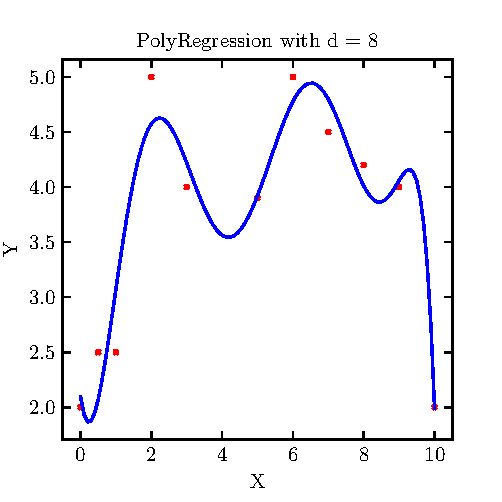
\includegraphics[width=\linewidth]{A4.1.pdf}
        \end{subfigure}
        \hfill
        \begin{subfigure}{0.48\linewidth}
                \centering
                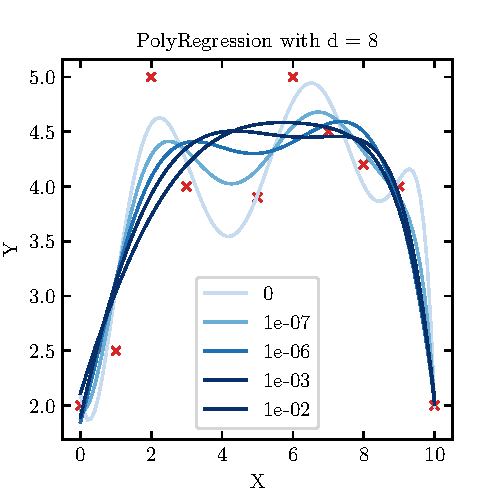
\includegraphics[width=\linewidth]{A4.2.pdf}
        \end{subfigure}
\end{figure}

Here is the code from \texttt{polyreg.py}:
\begin{minted}{python}
class PolynomialRegression:

        def __init__(self, degree=1, reg_lambda=1E-8):
                """
                Constructor
                """
                self.degree = degree
                self.regLambda = reg_lambda
                self.theta = None
                self.Xmean = None
                self.Xstd = None

        def polyfeatures(self, X, degree):
                """
                Expands the given X into an n * d array of polynomial features of
                        degree d.

                Returns:
                        A n-by-d numpy array, with each row comprising of
                        X, X * X, X ** 3, ... up to the dth power of X.
                        Note that the returned matrix will not include the zero-th power.

                Arguments:
                        X is an n-by-1 column numpy array
                        degree is a positive integer
                """
                X_ = X.flatten()
                degree_ = np.arange(1, degree+1) # array of polynomial exponents 1 -> degree
                return np.power.outer(X_, degree_) # return polynomial features

        def fit(self, X, y):
                """
                Trains the model
                Arguments:
                X is a n-by-1 array
                y is an n-by-1 array
                Returns:
                No return value
                Note:
                You need to apply polynomial expansion and scaling
                at first
                """
                n = len(X)
                
                # matrix of polynomial features
                X_ = self.polyfeatures(X, self.degree)
                # standardize features
                self.Xmean = X_.mean(axis=0)
                self.Xstd = X_.std(axis=0)
                X_ = (X_ - self.Xmean) / self.Xstd
                # add column of ones to front, for x^0
                X_ = np.c_[np.ones(n), X_]

                # regularization matrix
                regMatrix = self.regLambda * np.identity(self.degree + 1)
                regMatrix[0, 0] = 0

                # analytic solution (X'X + regMatrix)^-1 X' y
                self.theta = np.linalg.pinv(X_.T.dot(X_) + regMatrix).dot(X_.T).dot(y)

        def predict(self, X):
                """
                Use the trained model to predict values for each instance in X
                Arguments:
                        X is a n-by-1 numpy array
                Returns:
                        an n-by-1 numpy array of the predictions
                """
                n = len(X)

                # matrix of polynomial features
                X_ = self.polyfeatures(X, self.degree)
                # standardize features
                X_ = (X_ - self.Xmean) / self.Xstd
                # add column of ones to front, for x^0
                X_ = np.c_[np.ones(n), X_]

                return X_ @ self.theta
\end{minted}

Here is the code to make the plot with many different values of $\lambda$:
\begin{minted}{python}
# load the data
filePath = "data/polydata.dat"
file = open(filePath,'r')
allData = np.loadtxt(file, delimiter=',')

X = allData[:, [0]]
y = allData[:, [1]]

# plot curve
fig = plt.figure()
plt.plot(X, y, 'C3x', markersize=4)

# regression with degree = d
d = 8

# different lambdas to plots
lambdas = [0, 1e-7, 1e-6, 1e-3, 1e-2]
labels = ['0', '1e-07', '1e-06', '1e-03', '1e-02']

# colors for different lambdas
c = np.arange(len(lambdas))
norm = mpl.colors.Normalize(vmin=c.min(), vmax=c.max())
cmap = mpl.cm.ScalarMappable(norm=norm, cmap=mpl.cm.Blues)
cmap.set_array([])

for i in range(len(lambdas)):
    model = PolynomialRegression(degree=d, reg_lambda=lambdas[i])
    model.fit(X, y)
    xpoints = np.linspace(np.max(X), np.min(X), 100).reshape(-1, 1)
    ypoints = model.predict(xpoints)
    plt.plot(xpoints, ypoints, label=labels[i], c=cmap.to_rgba(i + 1))
    

plt.legend()
plt.title('PolyRegression with d = '+str(d))
plt.xlabel('X')
plt.ylabel('Y')
plt.show()

fig.savefig('../A4.2.pdf')
\end{minted}

\newpage

\textbf{A.5}

Here are the training curves.
The results match the plot in the problem statement.

\vspace{-0.1cm}
\hspace{-3.4cm}
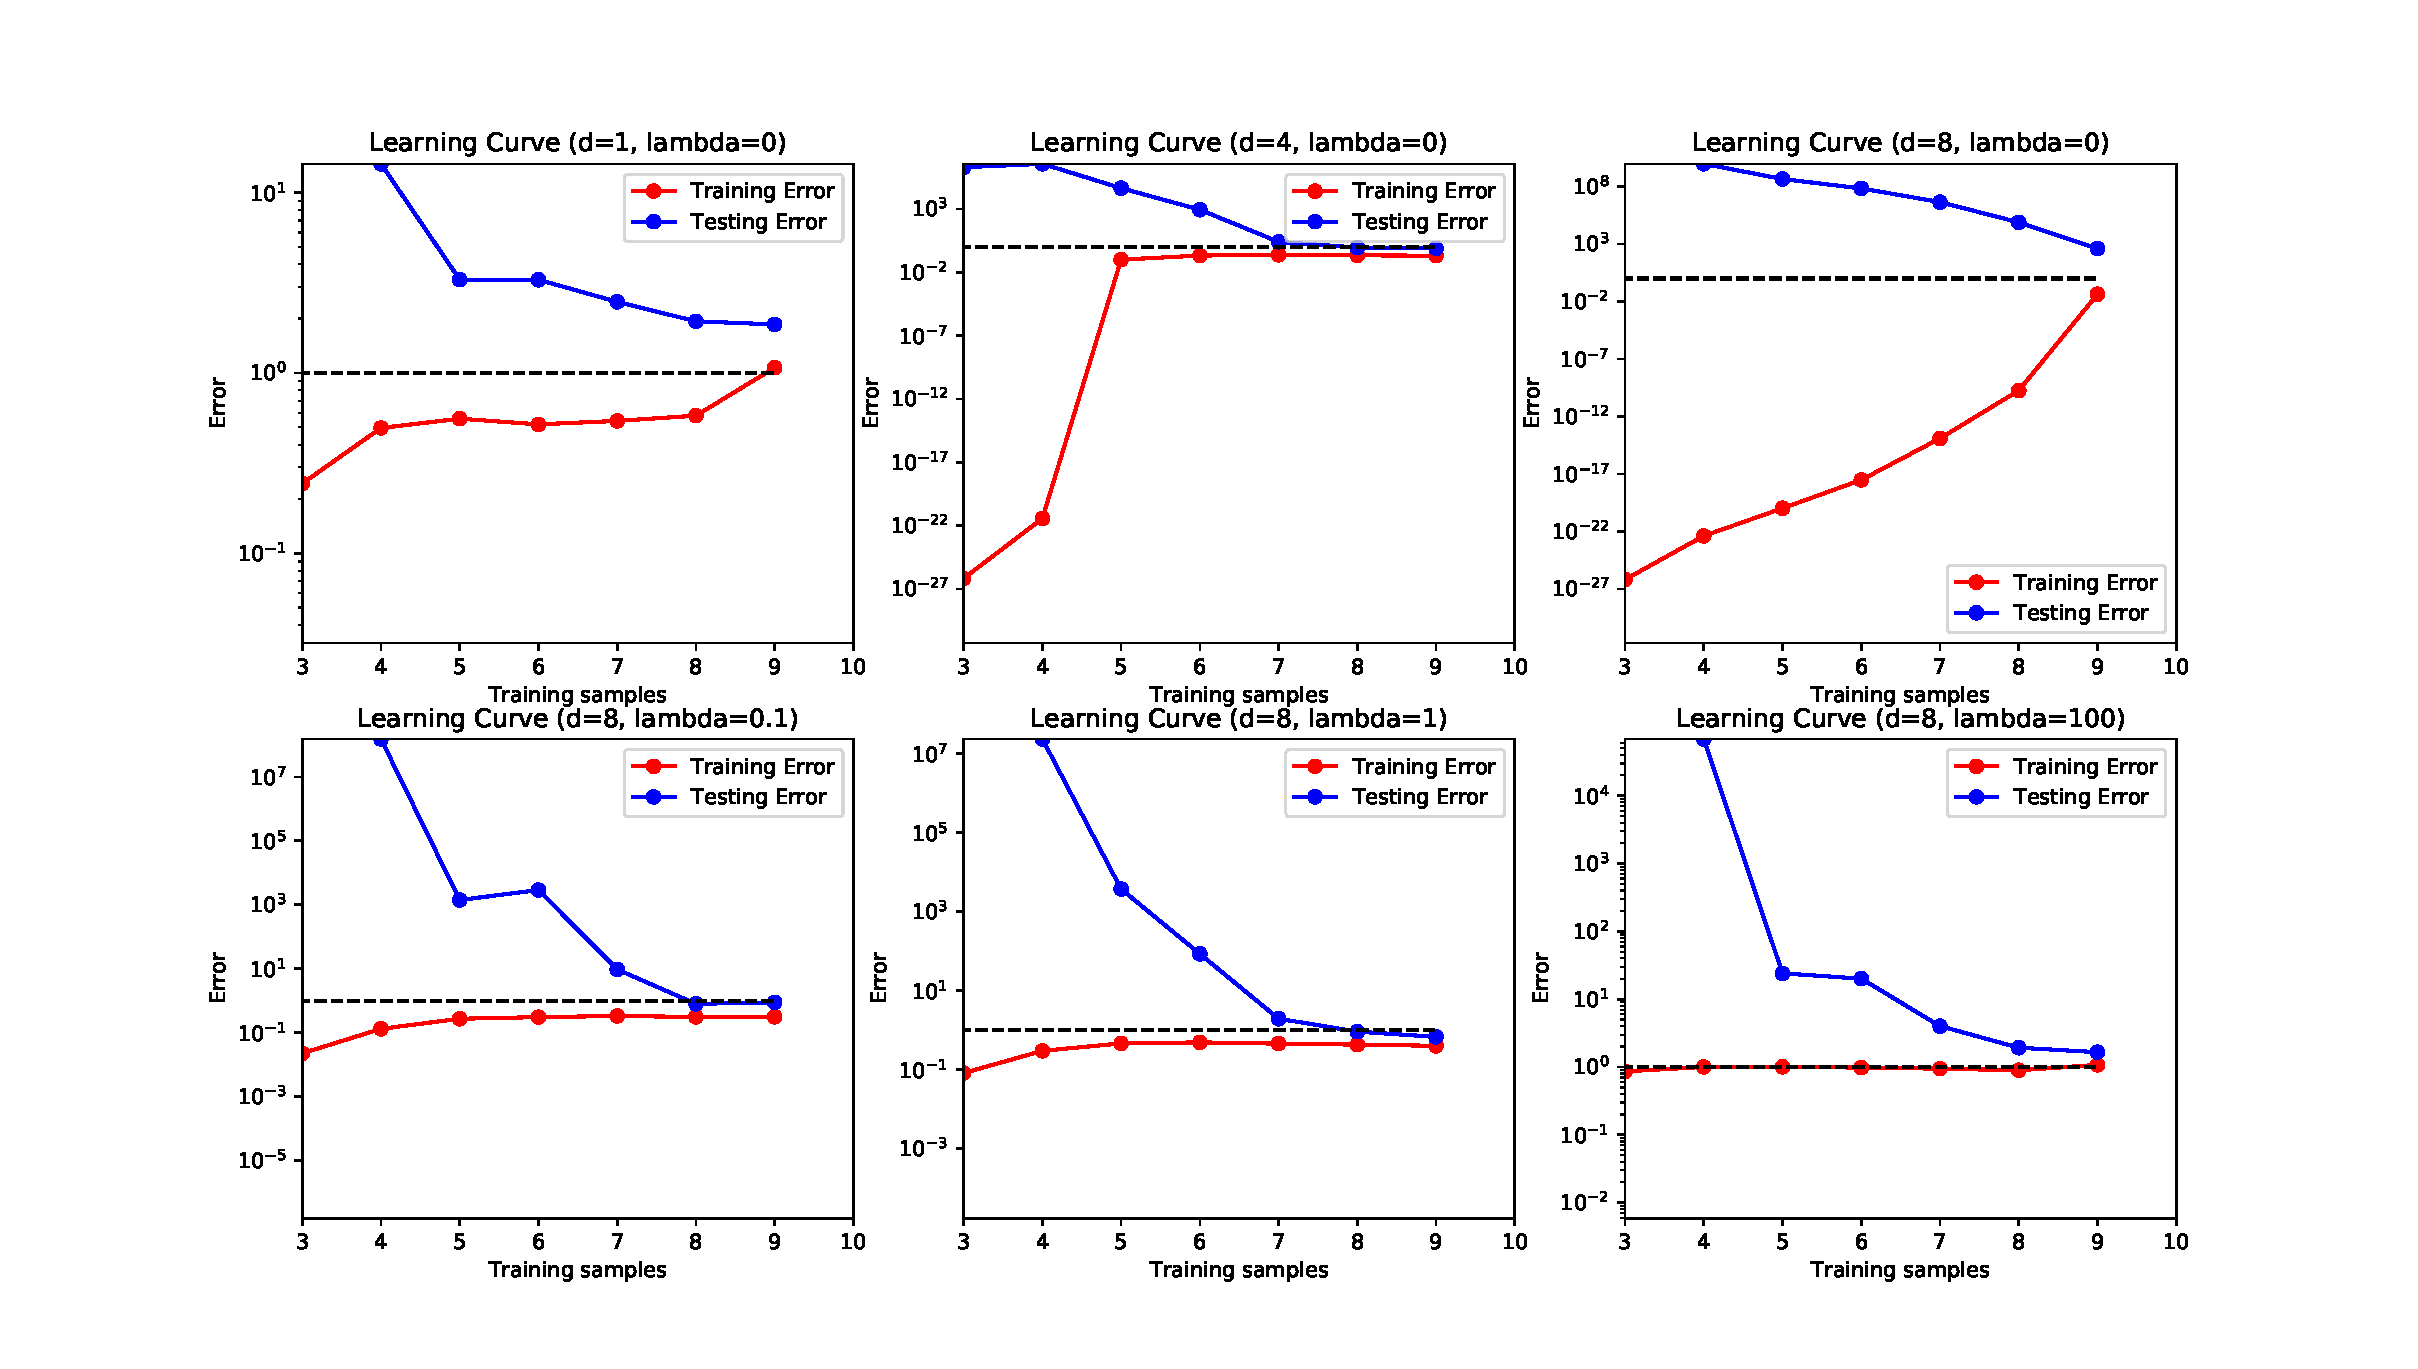
\includegraphics[width=1.4\textwidth]{A5.pdf}

\begin{minted}{python}
def learningCurve(Xtrain, Ytrain, Xtest, Ytest, reg_lambda, degree):
    """
    Compute learning curve

    Arguments:
        Xtrain -- Training X, n-by-1 matrix
        Ytrain -- Training y, n-by-1 matrix
        Xtest -- Testing X, m-by-1 matrix
        Ytest -- Testing Y, m-by-1 matrix
        regLambda -- regularization factor
        degree -- polynomial degree

    Returns:
        errorTrain -- errorTrain[i] is the training accuracy using
        model trained by Xtrain[0:(i+1)]
        errorTest -- errorTrain[i] is the testing accuracy using
        model trained by Xtrain[0:(i+1)]

    Note:
        errorTrain[0:1] and errorTest[0:1] won't actually matter, 
        since we start displaying the learning curve at n = 2 (or higher)
    """

    n = len(Xtrain)

    errorTrain = np.zeros(n)
    errorTest = np.zeros(n)

    for i in range(1,n):

        # fit on the first i training points
        model = PolynomialRegression(degree=degree, reg_lambda=reg_lambda)
        model.fit(Xtrain[:i+1], Ytrain[:i+1])

        # predict on first i training points and compute error
        Ytrain_pred = model.predict(Xtrain[:i+1])
        errorTrain[i] = np.mean((Ytrain[:i+1] - Ytrain_pred)**2)

        # predict on whole test set and compute error
        Ytest_pred = model.predict(Xtest)
        errorTest[i] = np.mean((Ytest - Ytest_pred)**2)

    return errorTrain, errorTest
\end{minted}

\newpage

\section*{Ridge Regression on MNIST}

\textbf{A.6}

\begin{enumerate}
        \item
        We can write the given equation as
        \begin{align*}
                \sum_{j=0}^k \left[ \norm{Xw_j - Ye_j}^2 + \lambda \norm{w_j}^2 \right]
                &= \sum_{j=0}^k \left[ (X w_j - Y e_j)^T (X w_j - Y e_j) + \lambda w_j^T w_j \right] \\
                &= \sum_{j=0}^k \left[ w_j^T X^T X w_j - w_j^T X^T y_j - y_j^T X w_j + y_j^T y_j + \lambda w_j^T w_j \right].
        \end{align*}
        Now taking the derivative with respect to vector $w_j$ and setting equal to zero, we have
        \begin{align*}
                \frac{\partial}{\partial w_j} [\,\cdots]
                &= \sum_{j=0}^k \left[ \hat{w}_j^T X^T X + \hat{w}_j^T X^T X - y_j^T X - y_j^T X + \lambda \hat{w}_j^T + \lambda \hat{w}_j^T \right] \\
                &= 2 \sum_{j=0}^k \left[ \hat{w}_j^T (X^T X + \lambda I) - y_j^T X \right]
                = 2 \sum_{j=0}^k \left[ (X^T X + \lambda I) \hat{w}_j - X^T y_j \right]^T = 0.
        \end{align*}
        We can now see that
        \begin{align*}
                \hat{w}_j = (X^T X + \lambda I)^{-1} X^T y_j,
        \end{align*}
        and as $w_j$ and $y_j$ are the columns of $W$ and $Y$, respectively, we have
        \begin{align*}
                \widehat{W} = (X^T X + \lambda I)^{-1} X^T Y
        \end{align*}

        \item
        I get $\hat{\epsilon}_\text{train} = 0.1423$ and $\hat{\epsilon}_\text{test} = 0.1397$ with the following code:
\begin{minted}{python}
import numpy as np
from mnist import MNIST

def load_dataset():
        mndata = MNIST('../../../python-mnist/data/')
        X_train, labels_train = map(np.array, mndata.load_training())
        X_test, labels_test = map(np.array, mndata.load_testing())
        X_train = X_train/255.0
        X_test = X_test/255.0

        return X_train, labels_train, X_test, labels_test

X_train, Y_train, X_test, Y_test = load_dataset()

class MNIST_Classifier():

        def __init__(self):
                self.W = None

        def train(self, X, Y, regLambda=0):
                
                n,d = X.shape
                
                # X matrix with ones column
                X_ = np.c_[np.ones(n), X]
                
                # regularization matrix
                regMatrix = regLambda * np.identity(d + 1)
                regMatrix[0, 0] = 0
                
                # Y matrix with one-hot encoding
                k = 10
                Y_ = np.identity(k)[Y]

                # analytical solution (X'X + regMatrix)^-1 X' Y
                self.W = np.linalg.solve(X_.T.dot(X_) + regMatrix, X_.T.dot(Y_))
                
        def predict(self, X):
                
                n,d = X.shape
                
                # X matrix with ones column
                X_ = np.c_[np.ones(n), X]
                
                # predict vectors
                Y = self.W.T.dot(X_.T).T
                
                # return argmax for each vector
                return Y.argmax(axis=1)

classifier = MNIST_Classifier()
classifier.train(X_train, Y_train, 1e-4)

diff_train = Y_train - classifier.predict(X_train)
e_train = len(diff_train[diff_train != 0]) / len(diff_train)
print(f'Train error = {e_train:.4f}')

diff_test = Y_test - classifier.predict(X_test)
e_test = len(diff_test[diff_test != 0]) / len(diff_test)
print(f'Test error = {e_test:.4f}')
\end{minted}
\end{enumerate}

\newpage

\textbf{B.2}
\begin{enumerate}
        \item \,
        \vspace{-7mm}
        \begin{center}
                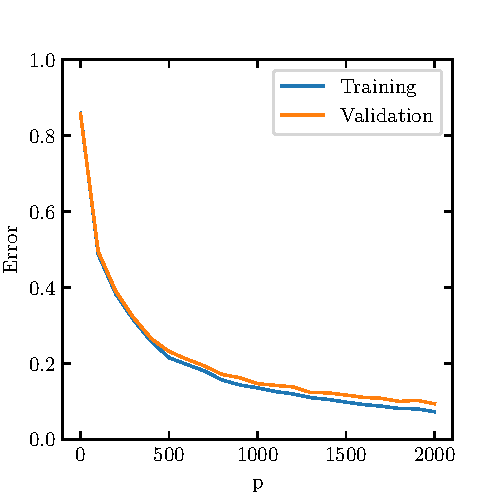
\includegraphics[width=0.5\linewidth]{code/B2a.pdf}
        \end{center}
        This plot was produced by the following code (which was run after the code listed in A.6.b):
        \begin{minted}{python}
np.random.seed(0)
# shuffle and split training set
idx_split = int(0.8 * len(X_train)) # where to split the set
idx_shuffle = np.random.permutation(np.arange(len(X_train))) # how to shuffle the set
X_train_new, X_val = X_train[idx_shuffle][:idx_split], X_train[idx_shuffle][idx_split:]
Y_train_new, Y_val = Y_train[idx_shuffle][:idx_split], Y_train[idx_shuffle][idx_split:]

# arrays to store errors
train_errs = []
val_errs = []

# loop over p
for p in np.arange(1,2002,100):
    
    # generate G and b
    G = np.random.normal(0, np.sqrt(0.1), (p,784))
    b = 2*np.pi * np.random.uniform(size=p)
    
    # calculate H
    H_train = np.cos((G @ X_train_new.T).T + b)
    H_val = np.cos((G @ X_val.T).T + b)
    
    # create a new classifier and train it
    classifier = MNIST_Classifier()
    classifier.train(H_train, Y_train_new, 1e-4)
    
    # calculate errors
    diff_train = Y_train_new - classifier.predict(H_train)
    e_train = len(diff_train[diff_train != 0]) / len(diff_train)
    train_errs.append(e_train)
    
    diff_val = Y_val - classifier.predict(H_val)
    e_val = len(diff_val[diff_val != 0]) / len(diff_val)
    val_errs.append(e_val)
    
    # print every 200 steps
    if p % 200 == 1:
        print(p)
        \end{minted}

        \item
        We can calculate the confidence interval by using the equalities in the given equation, and setting $\delta=0.05$.
        As the error can be anywhere in the range $[0,1]$, we have $a=0,~b=1$, and $m$ is the number of samples in the validation set, which is $12,000$.
        Plugging these values in, we get
        \begin{align*}
                \sqrt{\frac{(1-0)^2 \log(2/0.05)}{2 \cdot 12000}} \approx 0.012,
        \end{align*}
        assuming $\log$ is the natural logarithm.
        The best value of $p$ I tested was $p=2001$, for which the validation error was $0.093$.
        So we have $$\hat{\epsilon}_\text{test}(\hat{f}) = 0.093 \pm 0.012.$$
        Note that from the graph, it appears likely that with a better computer, you could go to higher values of $p$ and get even lower errors.
\end{enumerate}


\end{document}
